\documentclass[a4paper]{book} %{article}

\usepackage{fullpage} % Package to use full page
\usepackage{parskip} % Package to tweak paragraph skipping
\usepackage{tikz} % Package for drawing
\usepackage{amsmath}
\usepackage{hyperref}
\usepackage[numbered]{bookmark} % For numbering of challenges in bookmark pane of PDF viewer
\def\UrlBreaks{\do\/\do-}
\usepackage[absolute]{textpos}
\setlength{\TPHorizModule}{1mm}
\setlength{\TPVertModule}{1mm}
\usepackage{tikz}
\usepackage{siunitx}
\usepackage{datetime} % Time
\usepackage[UKenglish]{isodate}
\usepackage{ctable} % Thick table lines
\usepackage{booktabs} % Merge cells with multicolumn
\usepackage{bm} % Bold-maths \bm command

\newcommand{\courseyear}{2018 }
\newcommand{\disctime}{13:00 to 14:30 }
\newcommand{\discdays}{Mondays }
\newcommand{\discroom}{W4-766}
%\newcommand{\discexam}{10th February 2017}
\newcommand{\course}{Mechanics I }
\newcommand{\coursenospace}{Mechanics I}
\newcommand{\courseurl}{mechanics}
\newcommand{\nensei}{2nd}

\newcommand{\lap}[1]{\mathcal{L}\{#1\}}

\newcommand{\six}[1]{\SI[parse-numbers=false]{X}{#1}}
\newcommand{\com}[1]{\overline{#1}}
\newcommand{\hash}[2]{MD5(#1\_X) = #2\ldots}
\newcommand{\soltwodp}[2]{X = Your solution\\Form: Decimal to 2 decimal places.\\Place the indicated letter in front of the number.\\Example: aX where $X=46.00$ is entered as \href{http://www.wolframalpha.com/input/?i=md5+hash+of+\%22a46.00\%22}{a46.00}\\\\Hash of {#1}X = {#2}}

\graphicspath{{Images/}}

\begin{document}

\begin{titlepage}
    \begin{center}
        \vspace*{1cm}

        \Huge
        \textbf{Mechanics I}

        Spring quarter 2018

        \vspace{1.5cm}
        \Large
        Last updated:\\\today \ at \currenttime

        \vspace{4.0cm}
        \LARGE
        James Cannon\\Kyushu University
        \vfill

        \normalsize
        \url{http://www.jamescannon.net/teaching/\courseurl}\\
        \vspace{0.3cm}
        \small
        \url{http://raw.githubusercontent.com/NanoScaleDesign/Mechanics/master/mechanics_I.pdf}
        \vspace{0.5cm}

        License: \emph{CC BY-NC 4.0}.

    \end{center}
\end{titlepage}

\setcounter{chapter}{-1}

\tableofcontents

\chapter{Course information}
\newpage
\section{This course}
This is the Spring \courseyear \course course studied by \nensei-year undergraduate international students at Kyushu University.

\subsection{What you need to do}
\begin{itemize}
    \item Borrow the book ``Engineering Mechanics: Dynamics'', 6th edition, by Meriam and Kraige from the Mechanical Engineering office on the 4th floor of West 4. The course will be based on that book and you will need to refer to it in class.
    \item Prepare a challenge-log in the form of a workbook or folder where you can clearly write the calculations you perform to solve each challenge. This will be used in the final assessment and will be occasionally reviewed by the teacher.
    \item Submit a weekly feedback form by \textbf{9am on Monday} before class at \url{https://goo.gl/forms/ULjtgmL0Q2fZbG292}.
    \item Please bring a wifi-capable internet device to class, as well as headphones if you need to access online components of the course during class. If you let me know in advance, I can lend computers and provide power extension cables for those who require them (limited number).
\end{itemize}

\subsection{How this works}
\begin{itemize}
    \item This booklet forms part of an active-learning segment in the course. The learning is self-directed in contrast to the traditional lecture-style model.
    \item Learning is guided through solving a series of challenges combined with instant feedback about the correctness of your answer.
    \item There are no lectures. Instead, there is discussion time. Here, you are encouraged to discuss any issues with your peers, teacher and any teaching assistants. Furthermore, you are encouraged to help your peers who are having trouble understanding something that you have understood; by doing so you actually increase your own understanding too.
    \item Discussion-time is from \disctime on \discdays at room \discroom.
    \item Peer discussion is encouraged, however, if you have help to solve a challenge, always make sure you do understand the details yourself. You will need to be able to do this in an exam environment. The questions on the exam will be similar in nature to the challenges.
    \item Every challenge in the book typically contains a \textbf{Challenge} with suggested \textbf{Resources} which you are recommended to utilise in order to solve the challenge. Occasionally the teacher will provide extra \textbf{Comments} to help guide your thinking. A \textbf{Solution} is also made available for you to check your answer. Sometimes this solution will be given in encrypted form. For more information about encryption, see section \ref{sec:hashes}.
    \item For deep understanding, it is recommended to study the suggested resources beyond the minimum required to complete the challenge.
    \item The challenge document has many pages and is continuously being developed. Therefore it is advised to view the document on an electronic device rather than print it. The date on the front page denotes the version of the document. You will be notified by email when the document is updated. The content may differ from last-year's document.
    \item A target challenge will be set each week. This will set the pace of the course and defines the examinable material. It's ok if you can't quite reach the target challenge for a given week, but you should be careful not to fall behind, since the exam cannot be delayed.
    \item You may work ahead, even beyond the target challenge, if you so wish. This can build greater flexibility into your personal schedule, especially as you become busier towards the end of the semester.
    \item Your contributions to the course are strongly welcomed. If you come across resources that you found useful that were not listed by the teacher or points of friction that made solving a challenge difficult, please let the teacher know about it!
\end{itemize}

\subsection{Assessment}
In order to prove to outside parties that you have learned something from the course, we must perform summative assessments. You will receive a weighted score based on:

\begin{itemize}
    \item Challenge-log (10\%) - final state at the end of the course, showing your calculations for all the challenges in the course.
    %\item Coursework (20\%)
    \item Final exam (90\%)
\end{itemize}

Final score = MAX(Weighted score, Final exam)

%\newpage
\section{Coursework}
\course is a large subject with a wide-range of applications. This coursework is designed to give you the opportunity to follow your personal interest and investigate in depth an area of \course of your choice.

The task is as follows:

\textbf{1)} Create a document, explaining about any application of \course that interests you. The document should be \textbf{between 1 and 4 pages}, including any necessary figures, mathematics and references.

\textbf{2)} Create \textbf{1 to 2 challenge(s)} to accompany your report, so someone reading your document can test their knowledge.

\textbf{3)} Include \textbf{fully worked} solutions to challenges you make (ie, not only the final answer, but clearly show the steps involved in order to achieve the final answer).

\subsection{Submission}
Submission is electronic, and the file may be in any format, including PDF, LibreOffice, MS Word, Google docs, Latex, etc\ldots If you submit a PDF, please also submit the source-files used to generate the PDF.

Submit the materials by \textbf{email} to the teacher \textbf{before the class on 10 July 2017} with the subject ``[\coursenospace] Coursework''. I will confirm in the class that I received your coursework. If you cannot attend the class, you must request confirmation of receipt when you send the email.

Late submission:\\
By 23:59 on 11 July 2017: 90\% of the final mark.\\
By 23:59 on 17 July 2017: 50\% of the final mark.\\
Later submissions cannot be considered.

\subsection{Marking}
Marks will be assigned based on the degree to the report fulfills the following criteria:
For maximum marks you should do the following:
\begin{itemize}
    \item Clearly demonstrate your understanding of what you write about. You can do this by, for example, mathematically solving for a relevant case or explaining with words how it applies in different situations.
    \item Ensure your subject has some relation to Mechanics and is of Engineering relevance.
    \item Choose a subject that goes beyond the boundaries of the examples covered in the textbook.
    \item Ensure the work is your own and all references, images and text taken from other sources are properly cited.
    \item Pitch the description at a level appropriate level so that others in the class can follow your discussion.
    \item Explain in reasonable depth.
    \item Explain accurately and clearly.
\end{itemize}

\emph{Note: The application that you describe can does not have to be originally invented by you (although you are welcome to propose an application like this if you wish). The application may already exist, but you will need to demonstrate understanding about the application and calculations involved in the use of \course with this application.}

\newpage
\section{Timetable}

\begin{center}
    \begin{tabular}{|c|c|c|c|}
        \hline
        & \textbf{Discussion} & \textbf{Target} & \textbf{Note}          \\ \specialrule{.1em}{.05em}{.05em}
        \textbf{1}  & 10 April & -            &                          \\ \hline
        \textbf{2}  & 17 April & 1.4          &                          \\ \hline
        \textbf{3}  & 24 April & 1.7          &                          \\ \specialrule{.1em}{.05em}{.05em}    % 1.8 (rotation)
        \textbf{4}  & 8 May    & 1.12         &                          \\ \hline                              % momentum and other problems
        \textbf{5}  & 15 May   & 1.17         &                          \\ \hline                              % 4/6 part I (steady mass flow)
        \textbf{6}  & 22 May   &              &                          \\ \hline                              % 4/6 part II
        \textbf{7}  & 29 May   &              &                          \\ \specialrule{.1em}{.05em}{.05em}    % 4/7 part I (variable mass)
        \textbf{8}  & 5 June   &              &                          \\ \hline                              % 4/7 part II
        \textbf{9}  & 12 June  &              & Mid-term exam            \\ \hline                              % Mid-term exam?
        \textbf{10} & 19 June  &              &                          \\ \hline                              % Kinematics (7/2-7/5)
        \textbf{11} & 26 June  &              &                          \\ \specialrule{.1em}{.05em}{.05em}    % Kinematics general motion (7/6)
        \textbf{12} & 3 July   &              &                          \\ \hline
        \textbf{13} & 10 July  &              &                          \\ \hline
        \textbf{14} & 13 July  &              &                          \\ \hline                              % Legrange
        \textbf{15} & 24 July  & -            & Final exam               \\ \hline
    \end{tabular}
\end{center}

\newpage
\section{Hash-generation}
\label{sec:hashes}

Some solutions to challenges are encrypted using MD5 hashes. In order to check your solution, you need to generate its MD5 hash and compare it to that provided. MD5 hashes can be generated at the following sites:

\begin{itemize}
    \item Wolfram alpha: (For example: md5 hash of ``q1.00'') \url{http://www.wolframalpha.com/input/?i=md5+hash+of+\%22q1.00\%22}
    \item \url{www.md5hashgenerator.com}
\end{itemize}

Since MD5 hashes are very sensitive to even single-digit variation, you must enter the solution \emph{exactly}. This means maintaining a sufficient level of accuracy when developing your solution, and then entering the solution according to the format suggested by the question. Some special input methods:

\begin{center}
\begin{tabular}{|l|l|}
    \hline
    \textbf{Solution} & \textbf{Input} \\ \hline
    $5 \times 10^{-476}$ & 5.00e-476 \\
    $5.0009 \times 10^{-476}$ & 5.00e-476 \\
    $-\infty$ & -infinity (never ``infinite'')\\
    $2 \pi$ & $6.28$ \\
    i & im(1) \\
    2i & im(2) \\
    1 + 2i & re(1)im(2) \\
    -0.0002548 i & im(-2.55e-4) \\
    1/i = i/-1 = -i & im(-1) \\
    $e^{i2\pi}$ [$= cos(2 \pi) + isin(2 \pi) = 1 + i0 = 1$] & 1.00 \\
    $e^{i\pi/3}$ [$= cos(\pi/3) + isin(\pi/3) = 0.5 + i 0.87$] & re(0.50)im(0.87) \\
    Choices in order A, B, C, D & abcd \\
    \hline
\end{tabular}
\end{center}

The first 6 digits of the MD5 sum should match the first 6 digits of the given solution.


\chapter{Hash practise}
\section{Hash practise: Integer}

X = 46.3847\\
Form: Integer.\\
Place the indicated letter in front of the number.\\
Example: aX where $X=46$ is entered as \href{http://www.wolframalpha.com/input/?i=md5+hash+of+\%22a46\%22}{a46}

hash of aX = e77fac

\section{Hash practise: Decimal}

X = 49\\
Form: Two decimal places.\\
Place the indicated letter in front of the number.\\
Example: aX where $X=46.00$ is entered as \href{http://www.wolframalpha.com/input/?i=md5+hash+of+\%22a46.00\%22}{a46.00}

hash of bX = 82c9e7

\section{Hash practise: String}

X = abcdef\\
Form: String.\\
Place the indicated letter in front of the number.\\
Example: aX where $X=abc$ is entered as \href{http://www.wolframalpha.com/input/?i=md5+hash+of+\%22aabc\%22}{aabc}

hash of cX = 990ba0

\section{Hash practise: Scientific form}

X = 500,765.99\\
Form: Scientific notation with the mantissa in standard form to 2 decimal place and the exponent in integer form.\\
Place the indicated letter in front of the number.\\
Example: aX where $X=4 \times 10^{-3}$ is entered as \href{http://www.wolframalpha.com/input/?i=md5+hash+of+\%22a4.00e-3\%22}{a4.00e-3}

hash of dX = be8a0d


\chapter{Kinetics of systems of particles}
\newpage
\section{System centre-of-mass position, mass and velocity: I}

\subsection*{Resources}
\begin{itemize}
    \item Book sections 4/1 to 4/2
\end{itemize}


\subsection*{Comment}
You may use the following text as an alternative explanation to that in the book.

\subsubsection{Introduction}
You are already largely familiar with the kinetics of a single particle.
The idea of this short course is to extend these principles to the motion of a general system of particles.
This will enable you to describe the motion of both rigid and non-rigid bodies and systems.

A rigid body is defined as a solid system of particles where the distance between the particles does not change with respect to time.
Examples of rigid-bodies are numerous, including many machines operating in the air, on land or under the sea, including rockets and spacecraft.
A non-rigid body can come in two forms:
\begin{itemize}
    \item A single solid body that changes shape over time, perhaps due to elastic or non-elastic deformations.
    \item A defined mass of liquid or gaseous particles flowing at a given rate. Important examples include air and fuel flowing through the turbine of an aircraft engine, the exhaust from the nozzle of a rocket, or water passing through a pump.
\end{itemize}

\subsubsection{Generalising Newton's 2nd law}
Here we extend Newton's second law of motion to cover a general mass system, modelled by considering $n$ particles each with mass $m_i$ bounded by a closed surface in space:

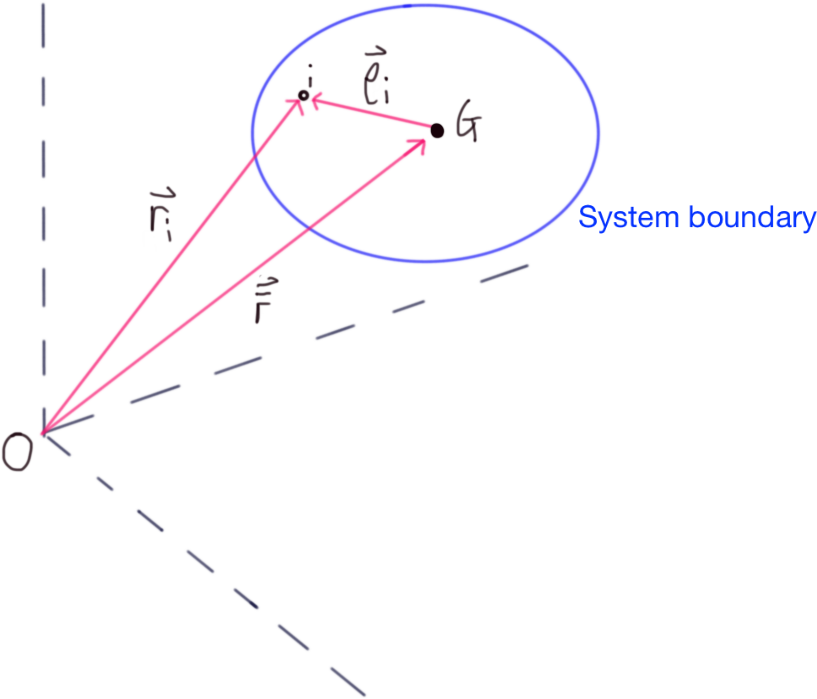
\includegraphics[width=8cm]{particle_system}

The centre-of-mass of the system is denoted by the point $G$ and the distance of particle $i$ from the centre-of-mass is $\bm{\rho_i}$. The distance of particle $i$ from an arbitrary non-accelerating origin $O$ of a Newtonian set of reference axes is $\bm{r_i}$ and the distance of the centre-of-mass from this origin is $\bm{\bar{r}}$. Note that point $G$ does not have to correspond to the position of any one particle, and may just represent the position of the centre-of-mass of the particles at that particular instant.

The total mass of the system $m$ is of course just sum of all the particle masses $m_i$:
\begin{equation}
    m = \sum{m_i}
\end{equation}

so that the centre-of-mass $G$ of the system can be determined from the position of all particles:
\begin{equation}
    m \bm{\bar{r}} = \sum m_i \bm{r}_i
\end{equation}

Each particular in the system is subject to forces. It is useful to group these forces into two contributions:
\begin{itemize}
    \item Sources internal to the system boundary (ie, other particles). For example, the force on particle $i$ by particle $j$.
    \item Sources external to the system boundary (eg, electric fields, gravity, etc).
\end{itemize}

One can consider the total force acting on the system as a whole. Note that the force on on particle $i$ by particle $j$ is equal and opposite to the force on particle $j$ by particle $i$. Thus the sum of forces from internal forces must all cancel out to be zero. If there are multiple external forces $\bm{F}_i$ on the system, then the total force on the system must be $\sum\bm{F}$. Thus the equation of motion for the system can be written as
\begin{equation}
    \label{eqn:generalnewton}
    \sum\bm{F} = m \bm{\bar{\ddot{r}}} = m \bm{\bar{a}}
\end{equation}
where $\bm{\bar{a}}$ corresponds to the acceleration of the centre-of-mass $G$.

Equation \ref{eqn:generalnewton} is the generalised form of Newton's second law of motion. Each component in a Cartesian system may be treated independently (eg, $\sum F_x = m \bar{a}_x$ etc). The resultant external force $\sum\bm{F}$ will have the same direction as the acceleration of the system $\bm{\bar{a}}$ at that instant of time, however the resultant external force does not necessarily pass through the centre-of-mass (usually it does not).


\subsection*{Challenge}
1. $\bm{\com{r}}$, $\dot{\bm{\com{r}}}$ and $\ddot{\bm{\com{r}}}$ of Question 4/1.

2. Question 4/4.

\subsection*{Solution}
1. Given in book.

2. \SI{534}{N}




\newpage
\section{System centre-of-mass position, mass and velocity: II}

\subsection*{Resources}
\begin{itemize}
    \item Book sections 4/1 to 4/2
\end{itemize}

\subsection*{Challenge}
Question 4/5. Determine the \emph{magnitude} of the acceleration.

\subsection*{Solution}
\SI{4}{m/s^2}




\newpage
\section{System centre-of-mass position, mass and velocity: III}

\subsection*{Resources}
\begin{itemize}
    \item Book sections 4/1 to 4/2
\end{itemize}

\subsection*{Challenge}
Question 4/13

\subsection*{Solution}
\SI{4.2}{m/s^2}




\newpage
\section{Kinetic and potential energy}

\subsection*{Resources}
\begin{itemize}
    \item Book section 4/3
\end{itemize}

\subsection*{Challenge}
1. Calculate $T$ in question 4/1

2. Question 4/10

\subsection*{Solution}
1. Given in book.

2. To check your final answer, substitute b = 2 metres into your final answer. You should obtain \SI{5.27}{m/s}.



\newpage
\section{Cross-product}

\subsection*{Resources}
\begin{itemize}
    \item \url{https://www.khanacademy.org/science/physics/magnetic-forces-and-magnetic-fields/electric-motors/v/calculating-dot-and-cross-products-with-unit-vector-notation}
\end{itemize}


\subsection*{Challenge}
1. Determine the angle between the two vectors $\bm{a} = [3,0,0]$ and $\bm{b} = [3,1,0]$ and use it to calculate $\bm{c} = \bm{a} \times \bm{b}$. Which direction does the vector $\bm{c}$ point?

2. Determine the cross product $\bm{f} = \bm{d} \times \bm{e}$ where $\bm{d} = 4 \hat{i}+ 2 \hat{j} + 1 \hat{k}$ and $\bm{e} = -2 \hat{i} -4 \hat{j} + 8 \hat{k}$ without calculating the angle between them.

\subsection*{Solution}
Please compare your answer with your partner and discuss in class if answers differ.




\newpage
\section{Rotation of particles I}

\subsection*{Resources}
\begin{itemize}
    \item Book section 4/4
\end{itemize}

\subsection*{Challenges}
Calculate the angular momentum and the rate of change of angular momentum with time for Question 4/1.

\subsection*{Solutions}
Given in book.



\newpage
\section{Rotation of particles II}

\subsection*{Resources}
\begin{itemize}
    \item Book section 4/4
\end{itemize}

\subsection*{Challenges}
Question 4/15

\subsection*{Solutions}
Given in book.




\newpage
\section{Rotation of particles III}

\subsection*{Resources}
\begin{itemize}
    \item Book section 4/4
\end{itemize}

\subsection*{Challenges}
Question 4/16

\subsection*{Solutions}
The required time should be \SI{2.72}{s}




\newpage
\section{Rotation of particles IV}

\subsection*{Resources}
\begin{itemize}
    \item Book section 4/4
\end{itemize}

\subsection*{Challenges}
Question 4/2

\subsection*{Solutions}
To check your answers substitute $d=2$ metres, $m=7$ kg, $v=3$ m/s and $f=7$ N into your final answers.
You should obtain
$\bm{H}_G = 432 \hat{i} + 144 \hat{j} + 168 \hat{k}$ \SI{}{kg m^2 /s}
and
$\dot{\bm{H}}_G = -8 \hat{i} - 12 \hat{j} + 0 \hat{k}$ \SI{}{Nm}




%\newpage
%\section{Conservation of momentum}
%
%\subsection*{Resources}
%\begin{itemize}
%    \item Book section 4/5
%\end{itemize}
%
%\subsection*{Challenges}
%1. In Question 4/17, at what point does the vehicle stop accelerating? % NT: Change this to calculating velocity first. Add a question about conservation of KE and PE before as well
%
%2. Solve Question 4/17
%
%3. Question 4/18
%
%\subsection*{Solutions}
%1. Please write your answer and compare with your partner in class
%
%2. Given in book
%
%3. 0.21 m/s




%\newpage
%\section{Conservation of momentum vs energy}
%
%\subsection*{Resources}
%\begin{itemize}
%    \item Book section 4/5
%\end{itemize}
%
%\subsection*{Challenges}
%1. Solve Question 4/19
%
%2. Why is energy not conserved here? Where did the energy go? Under what conditions is momentum conserved, and under what conditions is energy conserved?
%
%\subsection*{Solutions}
%1. Given in book
%
%2. Please write your answers and compare with your partner in class.




\newpage
\section{Energy and Rotation I}

\subsection*{Resources}
\begin{itemize}
    \item Book section 4/1 to 4/5
\end{itemize}

\subsection*{Challenge}
Solve Question 4/22.

\subsection*{Solution}
\SI{4.7}{m/s}



\newpage
\section{Energy and Rotation II}

\subsection*{Resources}
\begin{itemize}
    \item Book section 4/1 to 4/5
\end{itemize}

\subsection*{Challenge}
Solve Question 4/28

\subsection*{Solutions}
You should obtain an algebraic expression for $v$ and $\dot{\theta}$. To check your expression, you can substitute the following values into the expression:
$m_0=$ \SI{1}{\kg},
$v_0=$ \SI{1000}{\meter\per\second},
$b=$ \SI{1.5}{\meter} and
$m=$ \SI{4}{\kg}, whereby you should obtain
$v=$ \SI{111}{\meter\per\second} and
$\dot{\theta}=$ \SI{222}{\radian\per\second}.




%\newpage
%\section{In-plane flow}
%
%\subsection*{Resources}
%\begin{itemize}
%    \item Book section 4/6
%\end{itemize}
%
%\subsection*{Challenge}
%Derive equation 4/19 in the book from equation 4/19a.




%\newpage
%\section{Force on vane}
%
%\subsection*{Resources}
%\begin{itemize}
%    \item Book section 4/6
%\end{itemize}
%
%\subsection*{Challenge}
%Show your working for sample problem 4/5 (a) and (b)




%\newpage
%\section{Power and a vane}
%
%\subsection*{Resources}
%\begin{itemize}
%    \item Book section 4/6
%\end{itemize}
%
%\subsection*{Challenge}
%Considering sample problem 4/6,
%
%1. Explain in words what is meant by ``power by action of the fluid''.
%
%2. The power is defined here by measuring the force applied to move an object at a constant velocity. If force creates acceleration ($F=ma$), how can the velocity be constant?
%
%3. Work through and solve the sample problem.
%
%\subsection*{Solutions}
%Please compare your solutions with your partner. You may be asked to present your solutions to the class.




%\newpage
%\section{Balancing forces: Jet aeroplane example}
%
%\subsection*{Resources}
%\begin{itemize}
%    \item Book section 4/6
%\end{itemize}
%
%\subsection*{Challenge}
%Work through sample problem 4/8 to obtain the equation of motion of the system as given in the book ($m'_gu-m'_av=mg\sin{\theta}+D$).




%\newpage
%\section{Balancing forces: Jet aeroplane}
%
%\subsection*{Resources}
%\begin{itemize}
%    \item Book section 4/6
%\end{itemize}
%
%\subsection*{Challenge}
%Answer question 4/33.
%
%\subsection*{Solution}
%Given in book.



%\newpage
%\section{Balancing forces: Fire tug}
%
%\subsection*{Resources}
%\begin{itemize}
%    \item Book section 4/6
%\end{itemize}
%
%\subsection*{Challenge}
%Answer question 4/37.
%
%\subsection*{Solution}
%Given in book.




%\newpage
%\section{Balancing ball on a water stream}
%
%\subsection*{Resources}
%\begin{itemize}
%    \item Book section 4/6
%\end{itemize}
%
%\subsection*{Challenge}
%Answer question 4/42. Take note about the conservation of energy in the jet stream, and the fact that the jet stream remains intact. You can assume that the water stream is fully deflected horizontally when it hits the ball.
%
%\subsection*{Solution}
%\SI{4.8}{\meter}




%\newpage
%\section{Pressure I}
%
%\subsection*{Resources}
%\begin{itemize}
%    \item Book section 4/6
%\end{itemize}
%
%\subsection*{Challenge}
%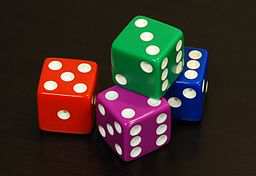
\includegraphics[width=4cm]{dice}
%
%A typical die has a side length of \SI{1.4}{\cm} and weighs \SI{2.8}{\gram}. Consider the die at rest on a desk. Estimate the pressure on the bottom of the die due to the desk.
%
%\subsection*{Solution}
%\SI{140}{\pascal}




%\newpage
%\section{Pressure II}
%
%\subsection*{Resources}
%\begin{itemize}
%    \item Book section 4/6
%\end{itemize}
%
%\subsection*{Challenge}
%Answer question 4/50
%
%\subsection*{Solution}
%\SI{1035}{\pascal}




%\newpage
%\section{Hose}
%
%\subsection*{Resources}
%\begin{itemize}
    %\item Book section 4/6
%\end{itemize}
%
%\subsection*{Challenge}
%Consider question 4/62. Note that the volume flow rate $Q$, measured in $m^3/s$, is the total system volume flow rate, and therefore the volume flow rate emerging from each nozzel is one quater of this for each nozzel.
%
%1. Write an expression for the velocity parallel and perpendicular to rotation for the case where $b$ tends to zero.
%
%2. Write an expression for the velocity parallel and perpendicular to rotation for the case where $r$ tends to zero.
%
%3. Remembering that components of angular velocity can be combined linearly independently, write an expression for the velocity parallel and perpendicular to rotation for the case where neither $b$ or $r$ are tending to zero.
%
%Answer question 4/62
%
%\subsection*{Solution}



%\newpage
%\section{Power and a Helicopter}
%
%\subsection*{Resources}
%\begin{itemize}
%    \item Book section 4/6
%\end{itemize}
%
%\subsection*{Challenge}
%Answer question 4/59
%
%\subsection*{Solutions}
%Given in book




%\newpage
%\section{Force components}
%
%\subsection*{Resources}
%\begin{itemize}
%    \item Book section 4/6
%\end{itemize}
%
%\subsection*{Challenge}
%Answer question 4/61
%
%\subsection*{Solutions}
%Given in book




\newpage
\section{Mass ejection}

\subsection*{Resources}
\begin{itemize}
    \item Book section 4/7
\end{itemize}

\subsection*{Challenge}
Consider rocket thrust where exhaust is emitted at a speed of \SI{220}{\meter\per\second}. The force on the rocket due to the thrust alone is \SI{400}{\newton}. Calculate (a) the mass flow rate $m'$ and (b) the time-rate increase of the mass of the rocket $\dot{m}$.

\subsection*{Solutions}
(a)\\
\soltwodp{a}{b54e89} (\SI{}{\kg\per\second})

(b)\\
\soltwodp{b}{6a83d8} (\SI{}{\kg\per\second})




\newpage
\section{Rocket sample problem}

\subsection*{Resources}
\begin{itemize}
    \item Book section 4/7
\end{itemize}

\subsection*{Challenge}
Complete the sample problem 4/11 using both solution I and II. Please be sure to follow the logic and understand the link between the two methods.




\newpage
\section{Rocket-style problem I}

\subsection*{Resources}
\begin{itemize}
    \item Book section 4/7
\end{itemize}

\subsection*{Challenge}
Answer question 4/67

\subsection*{Solution}
Given in book.




\newpage
\section{Rocket-style problem II}

\subsection*{Resources}
\begin{itemize}
    \item Book section 4/7
\end{itemize}

\subsection*{Challenge}
Answer question 4/82

\subsection*{Solution}
\SI{4.8}{\meter\per\second}




\newpage
\section{Mass intake I}

\subsection*{Resources}
\begin{itemize}
    \item Book section 4/7
\end{itemize}

\subsection*{Challenge}
Answer question 4/80

\subsection*{Solution}
\SI{1.6}{\meter\per\square\second} deceleration




\newpage
\section{Mass intake II}

\subsection*{Resources}
\begin{itemize}
    \item Book section 4/7
\end{itemize}

\subsection*{Challenge}
Answer question 4/76

\subsection*{Solution}
\SI{0.152}{\meter\per\square\second}




\newpage
\section{Chain style sample problem}

\subsection*{Resources}
\begin{itemize}
    \item Book section 4/7
\end{itemize}

\subsection*{Challenge}
Work through sample problem 4/9




\newpage
\section{Rope style sample problem}

\subsection*{Resources}
\begin{itemize}
    \item Book section 4/7
\end{itemize}

\subsection*{Challenge}
Work through sample problem 4/10




\newpage
\section{Chain vs Rope style sample problem difference}

\subsection*{Resources}
\begin{itemize}
    \item Book section 4/7
\end{itemize}

\subsection*{Challenge}
Considering the chain sample problem and the unconstrained rope problem, why was the kinetic energy different in these two cases? What assumptions were made in the chain problem compared to the unconstrained rope problem, and how did this impact the calculation of kinetic energy?

Please write a few sentences summarising your understanding.

\subsection*{Solution}
Please compare your writing with your partner's writing and discuss any differences.




\newpage
\section{Constrained and unconstrained rope style sample problem}

\subsection*{Resources}
\begin{itemize}
    \item Book section 4/7
\end{itemize}

\subsection*{Challenge}
Considering the unconstrained and constrained rope sample problem, how are the approaches different? How do the different values for ``P'' and ``R'' arise? What assumptions are different?

Please write a few sentences summarising your understanding.

\subsection*{Solution}
Please compare your writing with your partner's writing and discuss any differences.



\newpage
\section{Lifting a chain}

\subsection*{Resources}
\begin{itemize}
    \item Book section 4/7
\end{itemize}

\subsection*{Challenge}
An 18K gold chain has a mass of \SI{1.12}{\gram} and a length of \SI{40}{\cm}. You pick up one end of the chain and lift it up vertically at a constant velocity. There will be two downward forces present: one due to the hanging weight of the chain due to earth's gravity ($A$), and another induced by the constant addition of mass to the hanging part of the chain ($B$). If the chain is lifted up at \SI{5}{\cm\per\s}, calculate $B$. State what simplifying assumptions you make. How does this compare to $A$?

\subsection*{Solution}
$B$: \SI{7}{\micro\newton}




\newpage
\section{Chain on a pully}

\subsection*{Resources}
\begin{itemize}
    \item Book section 4/7
\end{itemize}

\subsection*{Challenge}
Answer question 4/83

\subsection*{Solution}
$P$ is given in book, and $R$ should match your understanding of the weight of the pile.




\newpage
\section{An accelerating chain}

\subsection*{Resources}
\begin{itemize}
    \item Book section 4/7
\end{itemize}

\subsection*{Challenge}
\textbf{a)} Consider a chain hanging over the edge of a block of height $h$. The chain has a total length $L$ and mass per unit length of $\rho$. At time t=0, the right end of the chain lays on top of the block at its right side at position x=0, while the left end of the chain is barely touching the ground. Initially the chain is stationary, but then the chain is released, causing the right side to accelerate horizontally in the left direction and the chain to pile up to the left of the block. Ignoring friction at the corner and making other idealised assumptions, obtain an expression for the acceleration of the chain as a function of the position of the end of the chain ($x$) as it slides along the horizontal surface, before it reaches the end of the block.

\textbf{b)} Did you need to consider the force generated by the stopping of the chain as it landed on the ground? If so, how did it come into the equation? If not, why not?

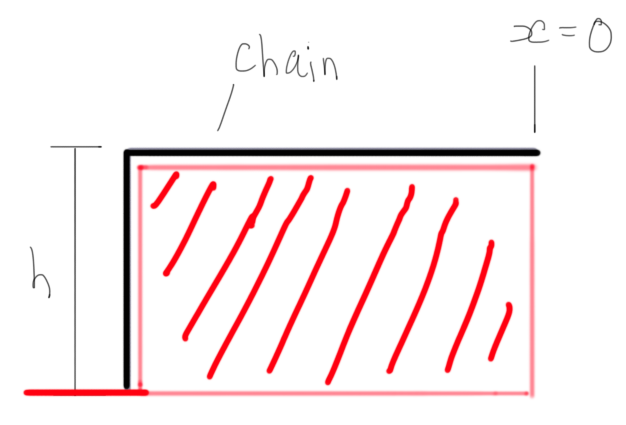
\includegraphics[height=5cm]{sliding_chain}

\subsection*{Solution}
\textbf{a)} To check your answer, determine the acceleration for a height of \SI{5}{\meter} and chain length of \SI{10}{\meter}, when the chain has slid \SI{2}{m}. You should obtain an acceleration of \SI{6.13}{\meter\per\square\second}.

\textbf{b)} Please discuss your answer with your partner



\newpage
\section{Making a question}

\fbox{\textbf{Coursework challenge}}

\subsection*{Resources}
\begin{itemize}
    \item Book section 4
\end{itemize}

\subsection*{Challenge}
Create an original question concerning anything covered in this chapter using the Peerwise platform (see section \ref{sec:peerwise} for details). If you create more than one question, the question awarded highest marks will be counted.

Your question must contain the following:
\begin{enumerate}
    \item A diagram to support your question.
    \item 5 possible answer options (A-E) that can be used by the student to check if their answer is correct. These may be numerical, mathematical, word-based or hashes.
    \item It is important that it is not possible to derive the method from the answer-options that you give.
    \item All the answer options should be plausible.
    \item For at least one of your wrong-answer options, ensure that the answer corresponds to a typical mistake that a student might make when answering your question. \label{lab:typical}
    \item Provide a detailed solution to your question, including explanation and mathematics. \emph{Demonstrate your own thinking and understanding.}
    \item Related to item \ref{lab:typical}, explain why the student might have chosen that wrong answer, and explain where they may have gone wrong in their thinking.
\end{enumerate}




\newpage
\section{Answering Peerwise question(s)}

\subsection*{Resources}
\begin{itemize}
    \item Book section 4
\end{itemize}

\subsection*{Challenge}
Choose at least one question from Peerwise and attempt to answer it.
Explain your reasoning (don't just write mathematics).
Clearly write an alternative explanation or possible improvement to the question you answered.

\subsection*{Solution}
Please discuss in class.


%\chapter{3D dynamics of rigid bodies}
%\newpage
\section{Radial velocity with horizontal connection}

\subsection*{Resources}
\begin{itemize}
    \item Book sections 7/1 to 7/5
\end{itemize}

\emph{Correction to book: Figure 7/9 should read $\bm{\alpha} = \bm{\dot{\omega}} = \bm{\Omega} \bm{\times} \bm{\omega}$ (not $\bm{\Omega} \bm{\times} \bm{r}$)}

\subsection*{Challenge}
A weight ``A'' is tethered to a pole by a stiff rod of length $r$. If the angular velocity is \SI{5.5}{\radian\per\second} $\hat{k}$ and the length of the rod is \SI{47}{\meter} along the x-axis, what is the linear velocity of the weight ``A''?

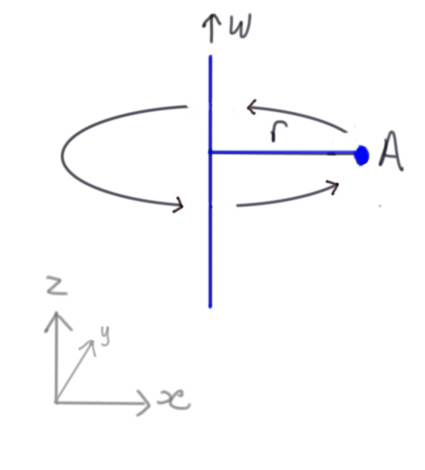
\includegraphics[height=5cm]{rod-horizontal}

\subsection*{Solution}
X = Your solution\\
Units: \si{\meter\per\second}\\
Form: Decimal, to 1 decimal place\\
Place the indicated letter in front of the number\\
Example: aX where $X=42.5$ \si{\meter\per\second} is entered as \href{http://www.wolframalpha.com/input/?i=md5+hash+of+\%22a42.5\%22}{a42.5}

$\hat{i}=$ hash of aX = 9497cd \si{\meter\per\second}\\
$\hat{j}=$ hash of bX = d17e5c \si{\meter\per\second}\\
$\hat{k}=$ hash of cX = 347133 \si{\meter\per\second}




\newpage
\section{Radial velocity with non-horizontal connection}

\subsection*{Resources}
\begin{itemize}
    \item Book sections 7/1 to 7/5
\end{itemize}

\emph{Correction to book: Figure 7/9 should read $\bm{\alpha} = \bm{\dot{\omega}} = \bm{\Omega} \bm{\times} \bm{\omega}$ (not $\bm{\Omega} \bm{\times} \bm{r}$)}

\subsection*{Challenge}
1. The position of ``A'' and the pole are unchanged (the radial distance is the same) and the angular velocity remains the same, but ``A'' is now hinged to the pole from below instead of horizontally, as shown in the picture. Calculate the linear velocity of ``A'' (calculate mathematically, not just by comparison with the previous challenge).

2. Write a sentence or two comparing your answer with that obtained from the previous challenge, including reasoning why.

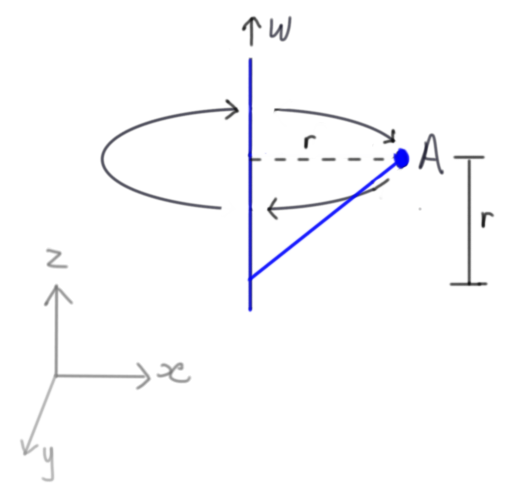
\includegraphics[height=5cm]{rod-frombelow}

\subsection*{Solution}
1.\\
X = Your solution\\
Units: \si{\meter\per\second}\\
Form: Decimal, to 1 decimal place\\
Place the indicated letter in front of the number\\
Example: aX where $X=42.5$ \si{\meter\per\second} is entered as \href{http://www.wolframalpha.com/input/?i=md5+hash+of+\%22a42.5\%22}{a42.5}

$\hat{i}=$ hash of dX = c6e675 \si{\meter\per\second}\\
$\hat{j}=$ hash of eX = bcff19 \si{\meter\per\second}\\
$\hat{k}=$ hash of fX = 979ed8 \si{\meter\per\second}

2. Please discuss in class if you are unsure about your answer.




\newpage
\section{Linear acceleration}

\subsection*{Resources}
\begin{itemize}
    \item Book sections 7/1 to 7/5
\end{itemize}

\emph{Correction to book: Figure 7/9 should read $\bm{\alpha} = \bm{\dot{\omega}} = \bm{\Omega} \bm{\times} \bm{\omega}$ (not $\bm{\Omega} \bm{\times} \bm{r}$)}

\subsection*{Challenge}
Using information from previous challenges, determine the:

1. Linear acceleration towards the centre of pole.

2. The tangential linear acceleration

3. Is there linear acceleration towards the centre of the pole? Is there tangential linear acceleration? Write a sentence or two to explain why for both cases.

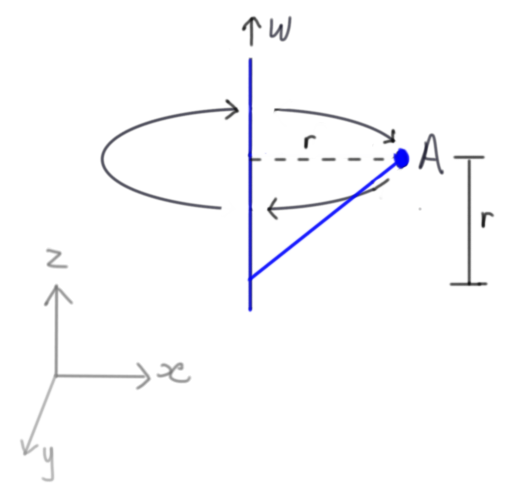
\includegraphics[height=5cm]{rod-frombelow}


\subsection*{Solution}
X = Your solution\\
Units: \si{\meter\per\square\second}\\
Form: Decimal, to 2 decimal place\\
Place the indicated letter in front of the number\\
Example: aX where $X=42.57$ \si{\meter\per\second} is entered as \href{http://www.wolframalpha.com/input/?i=md5+hash+of+\%22a42.5\%22}{a42.57}

1.\\
$\hat{i}=$ hash of gX = e1993f \si{\meter\per\square\second}\\
$\hat{j}=$ hash of hX = 5a16a7 \si{\meter\per\square\second}\\
$\hat{k}=$ hash of iX = 2ebd7c \si{\meter\per\square\second}

2.\\
$\hat{i}=$ hash of jX = 4b3090 \si{\meter\per\square\second}\\
$\hat{j}=$ hash of kX = 28435f \si{\meter\per\square\second}\\
$\hat{k}=$ hash of lX = 060ec3 \si{\meter\per\square\second}

3. Please compare your answer with your partner.




\newpage
\section{Radial acceleration - only magnitude}

\subsection*{Resources}
\begin{itemize}
    \item Book sections 7/1 to 7/5
\end{itemize}

\emph{Correction to book: Figure 7/9 should read $\bm{\alpha} = \bm{\dot{\omega}} = \bm{\Omega} \bm{\times} \bm{\omega}$ (not $\bm{\Omega} \bm{\times} \bm{r}$)}

\subsection*{Challenge}
Now consider that the radial velocity is not constant, but is undergoing an acceleration so that the magnitude of the angular velocity $\bm{w}$ increases while it continues to point in the same direction.

If the acceleration is \SI{2}{\radian\per\square\second}, what is the tangential acceleration of ``A''?

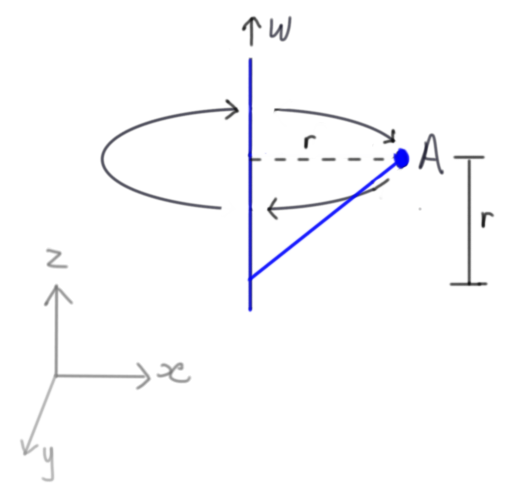
\includegraphics[height=5cm]{rod-frombelow}

\subsection*{Solution}
X = Your solution\\
Units: \si{\meter\per\second}\\
Form: Decimal, to 1 decimal place\\
Place the indicated letter in front of the number\\
Example: aX where $X=42.5$ \si{\meter\per\second} is entered as \href{http://www.wolframalpha.com/input/?i=md5+hash+of+\%22a42.5\%22}{a42.5}

$\hat{i}=$ hash of mX = b9f8f5 \si{\meter\per\second}\\
$\hat{j}=$ hash of nX = 57e394 \si{\meter\per\second}\\
$\hat{k}=$ hash of oX = 0c8b72 \si{\meter\per\second}





\newpage
\section{Radial acceleration - only direction (precession)}

\subsection*{Resources}
\begin{itemize}
    \item Book sections 7/1 to 7/5
\end{itemize}

\emph{Correction to book: Figure 7/9 should read $\bm{\alpha} = \bm{\dot{\omega}} = \bm{\Omega} \bm{\times} \bm{\omega}$ (not $\bm{\Omega} \bm{\times} \bm{r}$)}

\subsection*{Challenge}
The previous challenges considered the case (a) below, where the direction of the angular velocity vector $\omega$ was unchanging. Next consider that the angular velocity vector is precessing around an axis of symettry, and this precession has an angular velocity of $\Omega$, as shown in (b). Combining (a) and (b) we have (c).

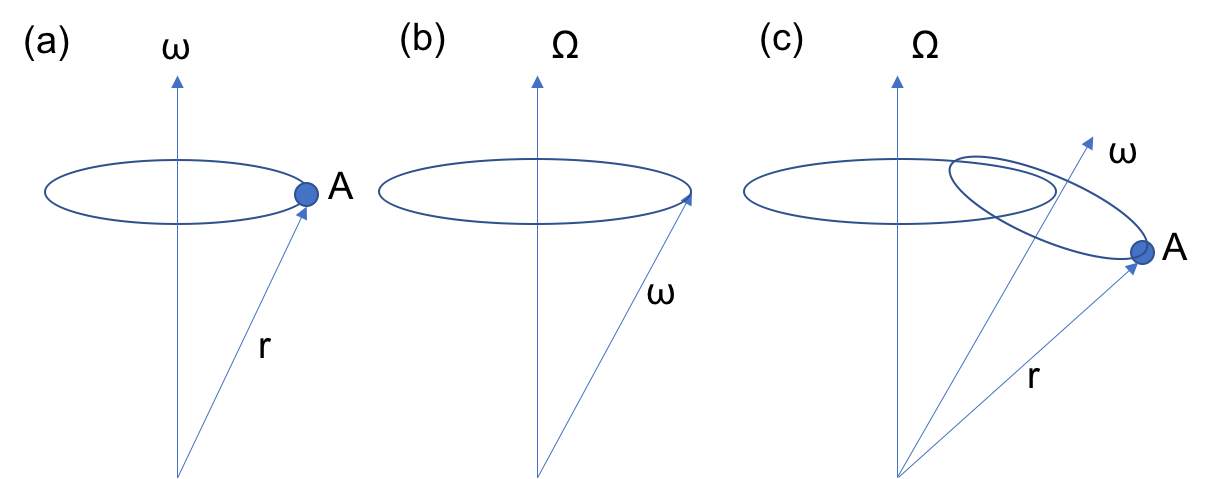
\includegraphics[height=5cm]{precession}

1. Consider the same system as before, but tilt the $\omega$ vector and allow the rotation to precess around a vector of symmetry $\Omega$. Assuming that only the direction (not the magnitude) of the angular velocity vector $\omega$ is changing with time, calculate the linear acceleration of ``A'' if $\Omega = 3\hat{k}$ \si{\radian\per\second} and angular velocity vector $\omega$ is inclined at \SI{45}{\degree} with components $\omega = 5.5 \hat{i} + 5.5 \hat{k}$. You may assume all other properties are the same as recent previous challenges.

2. What is the direction of the acceleration of the angular velocity vector $\omega$. Write 1 or 2 sentences to explain why.

3. What is the direction of the linear acceleration of ``A''. Write one or two sentences (possibly with a diagram) to explain when the sign will be opposite but with same magnitude.


\subsection*{Solution}
1. $-873 \hat{i} + 873 \hat{k}$

2. and 3. Please discuss in class.




\newpage
\section{Radial acceleration II}

\subsection*{Resources}
\begin{itemize}
    \item Book sections 7/1 to 7/5
\end{itemize}

\emph{Correction to book: Figure 7/9 should read $\bm{\alpha} = \bm{\dot{\omega}} = \bm{\Omega} \bm{\times} \bm{\omega}$ (not $\bm{\Omega} \bm{\times} \bm{r}$)}

\subsection*{Challenge}
Question 7/4

\subsection*{Solution}
\SI{1285}{\meter\per\second}


%\appendix 
%\chapter{Mid-term exam}
%\section{}

Briefly describe under what conditions the following are conserved. Give 1 example for each to support your writing. You do not need to write long calculations or more than a couple of sentences in order to achieve full marks for this question.

a) Momentum

b) Energy




\section{}

Consider the system of 2 particles below. At a given instant, one particle is positioned on the z-axis at a distance of $1.5d$ from the origin and has a mass of $4m$, travelling in the x direction at a constant velocity of $v$. The other particle is positioned on the x-axis at distance $d$ from the origin and has a mass of $m$, travelling in the $y$ direction with a velocity of $2v$ while experiencing a force $F$ in the z-direction.

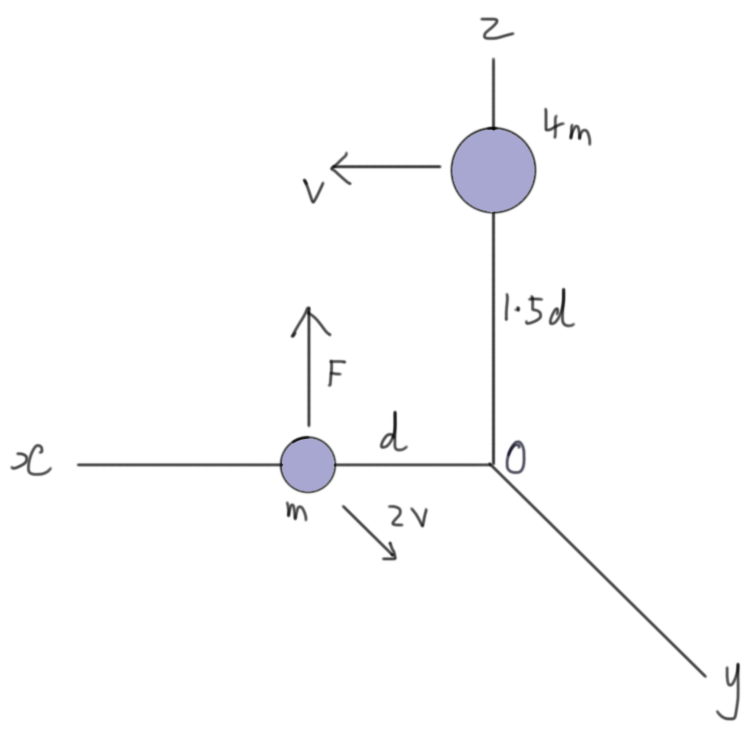
\includegraphics[height=7cm]{particles.png}

a) Determine the centre-of-mass position, velocity and acceleration.

b) Determine the angular momentum and torque about the origin ``O''.

c) Determine the angular momentum about the centre-of-mass of the system.




\section{}
An experimental hovercraft hovers just above the ground by pumping air at atmospheric pressure through the circular induct at $B$ with radius $r_B$ and discharging it horizontally under the skirt $C$ with radius $r_C$. Write an expression for the average air-pressure $P$ under the hovercraft, considering the balance of forces involved. You may consider the specific weight of air to be $\rho$ \si{\kg\per\cubic\meter} and the velocity of air entering the induct $B$ to be $v$ \si{\meter\per\second}.

\emph{Image taken from question 4/50 in book. Not included here for copyright reasons.}




\section{}
Consider a jet aircraft climbing at a constant velocity $v$ at an angle $\alpha$ as shown in the image.

\emph{Image taken from question 4/33 in book. Not included here for copyright reasons.}

Using appropriate simplifying assumptions,

a) Draw a force-balance diagram

b) Derive an expression to estimate the \emph{minimum} rate of fuel consumption required (mass of fuel per unit time) to achieve a climbing angle of $\alpha$.


\end{document}
